\documentclass[11pt]{article}

\usepackage[portuguese]{babel}
\usepackage[a4paper,top=2cm,bottom=2cm,left=3cm,right=3cm,marginparwidth=1.75cm]{geometry}
\usepackage{amsmath}
\usepackage{graphicx}
\usepackage{float}
\usepackage[colorlinks=true, allcolors=blue]{hyperref}
\usepackage{listings}
\usepackage{hyphenat}
\usepackage{xcolor}

\title{\textbf{MVP Cow8\\(Pesagem Semi-Automatizada de Gado)}}
\author{
    Renan da Silva Oliveira Andrade (\texttt{renan.silva3@pucpr.edu.br})\\
    Ricardo Lucas Kucek (\texttt{ricardo.kucek@pucpr.edu.br})\\
    Pedro Senes Velloso Ribeiro (\texttt{pedro.senes@pucpr.edu.br})\\ 
    Riscala Miguel Fadel Neto (\texttt{riscala.neto@pucpr.edu.br})\\
    Victor Valerio Fadel (\texttt{victor.fadel@pucpr.edu.br})
}

\begin{document}
\maketitle

\section{Descrição do contexto}

Em propriedades rurais, o controle de pesagem do rebanho é indispensável para a manutenção da qualidade de vida dos animais. Monitorar o peso de bovinos, equinos e outros animais implica avaliar o desempenho em relação ao ganho de peso, um aspecto de extrema relevância para a pecuária comercial, pois impacta diretamente na produtividade e na lucratividade.

O controle de pesagem permite avaliar e ajustar a distribuição alimentar dos animais, garantindo que se desenvolvam de forma saudável. Em propriedades que trabalham com equinos, como haras e fazendas de criação, a pesagem auxilia na divisão correta de alimentação, suplementos e medicações, evitando sub ou sobrepeso, o que pode comprometer a saúde e a performance desses animais.

Além disso, o controle periódico do peso pode indicar animais que perderam peso de forma mais acentuada que o usual, fator que pode alertar os criadores e cuidadores sobre possíveis doenças, evitando o agravamento do estado de saúde do animal ou a disseminação de doenças entre o rebanho. Isso permite uma intervenção precoce e um manejo sanitário mais eficiente.

Em síntese, o controle de pesagem dos animais reflete-se diretamente na qualidade de vida dos mesmos e na rentabilidade de propriedades rurais de cunho comercial.

\section{Problemática}
A pesagem manual de animais em propriedades rurais apresenta desafios como a necessidade de mão de obra especializada, o estresse causado aos animais e a possibilidade de erros humanos na coleta e registro dos dados. Além disso, a falta de um controle de pesagem eficiente pode resultar em uma nutrição não otimizada, comprometendo o crescimento e a saúde dos animais. Na pecuária comercial, a ausência de um monitoramento preciso do peso impacta diretamente na produtividade e na lucratividade, dificultando a identificação precoce de doenças e problemas nutricionais. A implementação de um sistema automatizado de pesagem torna-se essencial para garantir um manejo mais eficiente e melhorar a qualidade de vida dos animais.

\section{Motivação}
Apesar da importância do controle de peso dos animais, a pesagem na maioria das propriedades rurais de médio e pequeno porte ainda é realizada manualmente, exigindo mão de obra especializada para o registro de dados e o manejo dos animais. Esse método pode tornar a saúde dos animais vulnerável a possíveis erros no manejo e no controle das informações. Diante disto, um sistema semi-automatizado de pesagem e registro de dados aumentaria a eficiência dos recursos humanos e financeiros da propriedade, além de evitar problemas como a falta de confiabilidade dos dados, decorrente de erros humanos, e a necessidade de um meio físico para o armazenamento das informações.

\section{Proposta}
O controle de pesagem dos animais em propriedades rurais é essencial para garantir a saúde e a qualidade adequada dos bovinos, equinos e outros animais. A pesagem manual feita com mão de obra humana apresenta desafios, como a necessidade de mão de obra especializada, estresse nos animais e possíveis erros humanos. Assim, um sistema semi-automatizado de pesagem configura-se como uma solução eficiente para melhorar o manejo e a produtividade de criadouros.

\subsection{Descrição do Sistema}
O sistema proposto utilizará tecnologia NFC (\textit{Near Field Communication}) para a identificação individual dos animais e um mecanismo de controle para garantir que apenas um animal seja pesado por vez. Cada animal usará um colar ou brinco equipado com uma tag NFC única, permitindo seu cadastro e sua identificação por um sensor no momento da pesagem.

\subsection{Mecanismo de Pesagem}
O sistema contará com balanças eletrônicas fechadas por dois portões automatizados, que se abrirão assim que a pesagem for bem-sucedida. Antes da medição do peso, serão realizadas as seguintes verificações:

\begin{itemize}
    \item Verificação da tag NFC: Um operador do sistema identifica o animal pela sua tag utilizando um sensor e registra qual animal está sendo pesado.
    \item Verificação do peso: O peso detectado é tratado para garantir a consistência do peso medido.
\end{itemize}

Caso ambas as verificações sejam aprovadas, o peso do animal será mensurado e registrado, e os portões da balança se abrirão para uma nova pesagem. Caso contrário, um alerta sonoro será emitido para que um operador verifique o problema e restabeleça o funcionamento adequado da balança.

\subsection{Armazenamento e Acesso aos Dados}
As informações de cada pesagem, incluindo o ID da tag NFC do animal e seu peso, serão armazenadas em um banco de dados MySQL via integração dos sistemas embarcados e seus sensores com um broker MQTT. O acesso aos dados será feito por meio de uma aplicação web desenvolvida em Flask, que permitirá que os usuários:

\begin{itemize}
    \item Visualizem o peso individual de cada animal;
    \item Ordenem a lista de animais pelo peso;
    \item Visualizem a média de peso do rebanho;
    \item Recebam alertas automáticos caso haja variações e/ou anomalias no peso de animais.
\end{itemize}

\subsection{Suporte de navegação com Chat IA}
A aplicação contará com um chat com a integração de uma inteligência artificial LLM que terá acesso a base de dados e ao funcionamento do site, permitindo que os usuários interajam com o sistema de maneira intuitiva. Os usuários poderão acessar todas as informações do site por meio do chat, que interpretará a pergunta, analisará e disponibilizará a informação demandada sem a necessidade de um conhecimento técnico prévio.

O sistema de pesagem automática proporcionará um monitoramento eficiente e automatizado da saúde e do desenvolvimento dos animais, reduzindo erros, otimizando a nutrição e garantindo um manejo mais inteligente e produtivo na pecuária.

\section{Tecnologias envolvidas}
Para a construção do projeto físico, serão utilizados alguns componentes eletrônicos:

\textit{Os itens marcados com * representam itens usados para prototipação, podendo ser substituídos por componentes mais robustos em produção.}

\begin{itemize}
    \item 1 Microcontrolador ESP32;
    \item *1 Sensor NFC RFID-RC522;
    \item *Tags NFC Mifare 13.96 MHz
    \item *Células de carga strain gauge 50 kg;
    \item Módulo amplificador HX711;
    \item 1 Buzzer passivo;
    \item 2 Servo motores.
    \item *1 Protoboard.
\end{itemize}

Além destes itens, serão utilizados componentes padrão para o funcionamento eletrônico do projeto (resistores, jumpers, etc.).

Para a construção do projeto web, serão utilizadas tecnologias como:
\begin{itemize}
    \item Flask;
    \item SQLAlchemy;
    \item *Broker MQTT EMQX;
    \item HTML, CSS, JS.
\end{itemize}

Para o armazenamento dos dados, serão utilizadas tecnologias como:
\begin{itemize}
    \item MySQL;
    \item *Docker.
\end{itemize}


\section{Resultados esperados}
Espera-se que o sistema de pesagem automatizada proporcione os seguintes resultados:

\begin{itemize}
\item \textbf{Redução significativa de erros humanos no registro de pesos}:
A automação do processo de pesagem eliminará a necessidade de intervenção manual, reduzindo a probabilidade de erros na coleta e no registro dos dados. Isso garantirá maior confiabilidade nas informações, permitindo decisões mais precisas no manejo dos animais.

\item \textbf{Melhoria no manejo nutricional e sanitário dos animais}: 
Com dados precisos e atualizados sobre o peso dos animais, será possível ajustar a alimentação e a suplementação de forma individualizada, garantindo um desenvolvimento saudável e equilibrado. Além disso, a identificação precoce de variações de peso permitirá intervenções rápidas em casos de doenças ou desnutrição.

\item \textbf{Aumento da eficiência operacional, reduzindo a necessidade de mão de obra especializada}: 
A automação do processo de pesagem diminuirá a dependência de mão de obra especializada, reduzindo custos operacionais e otimizando o tempo dos funcionários, que poderão ser realocados para outras atividades prioritárias na propriedade.

\item \textbf{Identificação precoce de variações de peso que possam indicar problemas de saúde}: 
O sistema permitirá o monitoramento contínuo do peso dos animais, gerando alertas automáticos em caso de variações significativas. Isso facilitará a detecção precoce de doenças, problemas nutricionais ou estresse, contribuindo para um manejo sanitário mais eficiente.

\item \textbf{Integração eficiente dos dados coletados com uma aplicação web, permitindo acesso remoto e em tempo real às informações}: 
A integração dos dados coletados com uma plataforma web possibilitará o acesso remoto e em tempo real às informações de pesagem. Isso permitirá que produtores e veterinários acompanhem o desenvolvimento dos animais de qualquer localidade, facilitando a tomada de decisões estratégicas.

\item \textbf{Redução do estresse nos animais durante o processo de pesagem}: 
A automação do sistema minimizará a necessidade de contenção física e interação humana direta, reduzindo o estresse nos animais e contribuindo para seu bem-estar geral.

\item \textbf{Otimização da produtividade e lucratividade da propriedade}: 
Com um controle mais preciso do peso e da saúde dos animais, espera-se um aumento na produtividade do rebanho, refletindo diretamente na lucratividade da propriedade. A redução de custos com mão de obra e a prevenção de perdas por doenças também contribuirão para esse resultado.

\item \textbf{Facilidade de uso e acessibilidade para produtores rurais}: 
A inclusão de um chat com inteligência artificial na aplicação web permitirá que produtores rurais, mesmo sem conhecimento técnico avançado, interajam com o sistema de forma intuitiva, acessando informações e relatórios de maneira simplificada.

\item \textbf{Base de dados histórica para análises futuras}: 
O armazenamento contínuo dos dados de pesagem em um banco de dados MySQL permitirá a criação de um histórico completo do desenvolvimento dos animais. Esses dados poderão ser utilizados para análises estatísticas, planejamento de melhorias no manejo e tomada de decisões estratégicas a longo prazo.
\end{itemize}

\section{Cronograma}
O cronograma do projeto está dividido em etapas, incluindo a aquisição de componentes, desenvolvimento do hardware e software, testes e implementação. A Figura 1 ilustra o planejamento detalhado.

\begin{figure}[H]
    \centering
    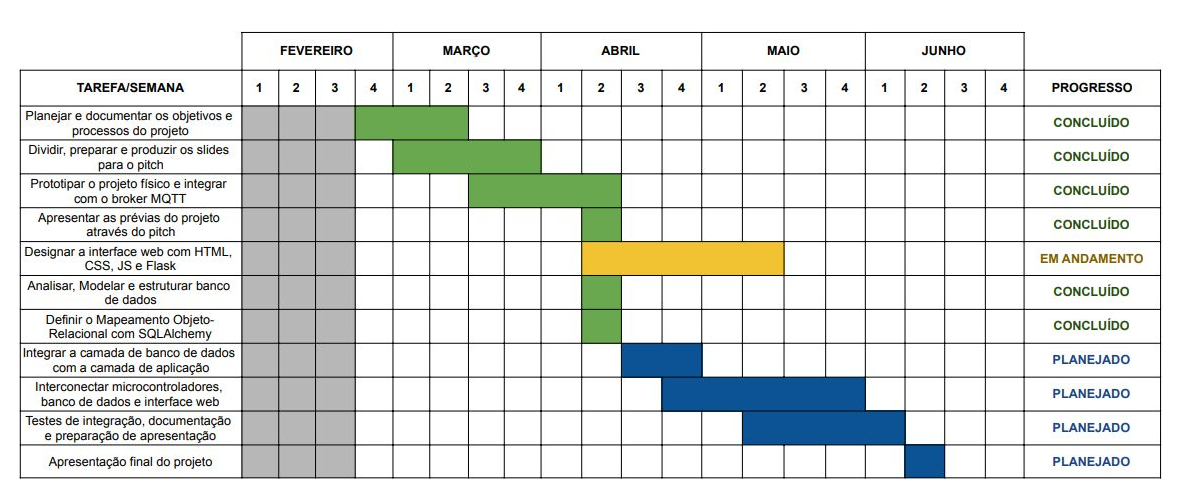
\includegraphics[width=0.9\linewidth]{cronograma.png}
    \caption{Cronograma}
\end{figure}

\section{Diretrizes para o Uso de IA}

Durante a preparação desta documentação, o(s) autor(es) usaram Chat DeepSeek V3 para correções ortográficas e verificação de conformidade e legitimidade dos dados. Após usar essa ferramenta, o(s) autor(es) revisaram e editaram o conteúdo conforme necessário e assumem total responsabilidade pelo conteúdo.

% \bibliographystyle{apalike}
% \bibliography{sample}

\end{document}
